\documentclass[xcolor=x11names, compress]{beamer}

\definecolor{CoolBlack}{rgb}{0.0, 0.18, 0.39}
\definecolor{byellow}{rgb}{0.55037, 0.38821, 0.06142}

\usepackage[T1]{fontenc}
\usepackage[utf8]{inputenc}
\usepackage{lmodern}
\usepackage{amsthm}
\usepackage{amssymb}
\usepackage{amstext}
\usepackage{bm}
\usepackage{graphicx}
\usepackage{epstopdf}
\usepackage{amsmath}
\usepackage{setspace}
\usepackage{tikz}
\usepackage{Tabbing}
\usepackage{mathrsfs}
\usepackage[mathcal]{euscript}
\usepackage{	epsfig}
\usepackage{changepage}
\usepackage{xcolor}
\usepackage{fancyvrb}
\usepackage{caption}
\usepackage{color}
\usepackage[version=3]{mhchem}
\usepackage{hyperref}
\usepackage{multirow}
\usepackage[firstpage]{draftwatermark}
\usepackage{animate}
\usepackage{appendixnumberbeamer}


\usetikzlibrary{decorations.fractals}

\setbeamerfont{title like}{shape=\scshape}
\setbeamerfont{frametitle}{shape=\scshape}

\setbeamercolor*{lower separation line head}{bg=CoolBlack}
\setbeamercolor*{normal text}{fg=black,bg=white}
\setbeamercolor*{alerted text}{fg=dgreen} 
\setbeamercolor*{example text}{fg=black}
\setbeamercolor*{structure}{fg=black}

% Margins
\mode<presentation>
{
  \definecolor{berkeleyblue}{HTML}{003262}
  \definecolor{berkeleygold}{HTML}{FDB515}
  \usetheme{Boadilla}      % or try Darmstadt, Madrid, Warsaw, Boadilla...
  %\usecolortheme{dove} % or try albatross, beaver, crane, ...
  \setbeamercolor{structure}{fg=berkeleyblue,bg=berkeleygold}
  \setbeamercolor{palette primary}{fg=berkeleyblue,bg=berkeleygold}
  \setbeamercolor{palette secondary}{fg=berkeleyblue,bg=berkeleygold}
  \setbeamercolor{palette tertiary}{bg=berkeleyblue,fg=white}
  \usefonttheme{structurebold}  % or try serif, structurebold, ...
  \useinnertheme{circles}
  \setbeamertemplate{caption}[numbered]
  \usebackgroundtemplate{}
}

%% Beamer Layout %%%%%%%%%%%%%%%%%%%%%%%%%%%%%
\useoutertheme[subsection=false,shadow]{miniframes}
%\useinnertheme{default}
%\usefonttheme{serif}
%\usepackage{palatino}
%\usepackage{tabu}

% addition of color
\definecolor{dgreen}{rgb}{0.,0.6,0.}
\definecolor{RawSienna}{cmyk}{0,0.72,1,0.45}

%\usepackage[sorting=none]{biblatex}
\mode<presentation>

% Links
\definecolor{links}{HTML}{003262}
\hypersetup{colorlinks,linkcolor=,urlcolor=links}

% columns
\renewcommand{\(}{\begin{columns}}
\renewcommand{\)}{\end{columns}}
\newcommand{\<}[1]{\begin{column}{#1}}
\renewcommand{\>}{\end{column}}

\def\bal#1\nal{\begin{align}#1\end{align}}
\def\bala#1\nala{\begin{align*}#1\end{align*}}
\def\bsub#1\nsub{\begin{subequations}#1\end{subequations}}
\newcommand{\f}{\frac}
\newcommand{\ux}{{\bm x}}
\newcommand{\un}{{\bm n}}
\newcommand{\unab}{{\bf \nabla}}
\newcommand{\bg}{\big>}
\newcommand{\bl}{\big<}
\newcommand{\su}{\big< s\big>}
\newcommand{\sd}{\big< s^2\big>}
\newcommand{\st}{\big< s^3\big>}
\newcommand{\sq}{\big< s^4\big>}
\renewcommand{\sc}{\big< s^5\big>}
\renewcommand{\ss}{\big< s^6\big>}
\newcommand{\sue}{\big< s\big>_\epsilon}
\newcommand{\sde}{\big< s^2\big>_\epsilon}
\newcommand{\ste}{\big< s^3\big>_\epsilon}
\newcommand{\sqe}{\big< s^4\big>_\epsilon}
\newcommand{\sce}{\big< s^5\big>_\epsilon}
\newcommand{\sse}{\big< s^6\big>_\epsilon}
\newcommand{\wsa}{\widehat\Sigma_a}
\newcommand{\wst}{\widehat\Sigma_t}
\newcommand{\wq}{\widehat Q}
\newcommand{\ep}{\varepsilon}
\newcommand{\vi}{{\varphi}}
\newcommand{\uom}{{\bm\Omega}}
\newcommand{\setb}{\mathcal{B}}


\SetWatermarkText{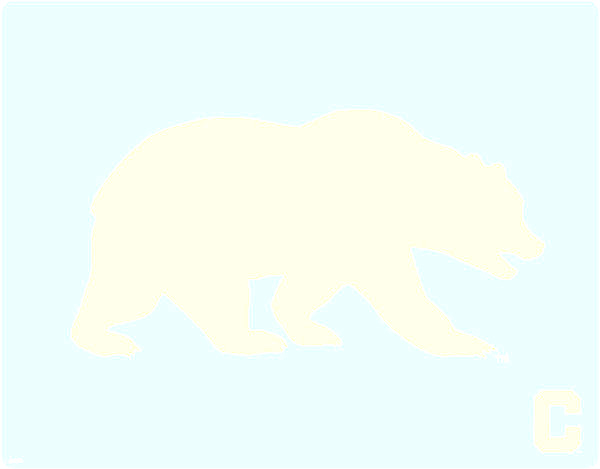
\includegraphics{images/watermark_calbear.jpg}}
\SetWatermarkAngle{0}
\SetWatermarkScale{0.61}

\title{1-D Nonclassical Diffusion }
\author{Vasques, Slaybaugh}
\date{October 31, 2016}

%%%%%%%%%%%%%%%%%%%%%%%%%%%%%%%%%%%%%%%%%%%%%%%%%%

\begin{document}

%%%%%%%%%%%%%%%%%%%%%%%%%%%%%%%%%%%%%%%%%%%%%%%%%%%%%%

%SLIDE1 TITLE---------------------------------------------------------------------------------
\begin{frame}[plain]
\title{Simplified P$_N$ Equations for Nonclassical Transport with Isotropic Scattering}
\author{
\begin{tabular}{ccc}
\multirow{6}{65pt}{
\includegraphics[height=2.5cm]{images/title_bk.eps}}
& &
\multirow{6}{65pt}{
\includegraphics[height=2.5cm]{images/title_bk.eps}} \\
&{\small\textcolor{blue}{University of California, Berkeley}} &\\
&{\small\textcolor{blue}{Department of Nuclear Engineering}}&\\
&{\small \textcolor{blue}{Neutronics Research Group}}&\\
& &\\
&\textbf{Richard Vasques}&\\
&\textbf{Rachel N. Slaybaugh}&\\
%&\textbf{ }&\vspace{-10pt}\\
%&\textbf{Kai Krycki$^1$}&\\
%CO-AUTHOR'S INSTITUTION
%\multicolumn{3}{c}{\small\textcolor{blue}{$^1$Aachen Institute for Nuclear Training GmbH}}
\end{tabular}}
\date{DATE, 2017 \\ M\&C 2017, Jeju, Korea}
\titlepage
\end{frame}


%%%%%%%%%%%%%%%%%%%%%%%%%%%%%%%%%%%%%%%%%%%%%%%%%%%%%%
\section{\scshape Classical vs. Nonclassical}

%SLIDE2--------------------------------------------------------------------------------
\frame[c]{
	\frametitle{In classical transport}

	The ``colliders'' in the background material are, in general, \textbf{Poisson-distributed}; that is, their spatial locations are \textbf{not} correlated.\\
	\vspace{15pt}

\begin{center}
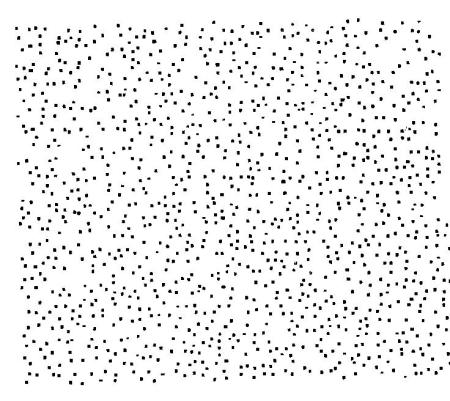
\includegraphics[scale=0.5,angle=0]{images/01-fig.jpg}\textcolor{white}{space}
%\pause
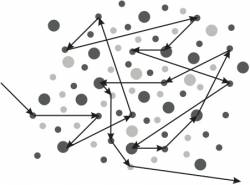
\includegraphics[scale=0.5]{images/02-fig}
\end{center}
\begin{block}{}	Specifically, this implies that the probability distribution function \textcolor{blue}{$p(s)$} for particles' \textbf{distances-to-collision} \textcolor{blue}{$s$} (free-paths) is given by an exponential:
	\[
	\textcolor{blue}{
	p(s) = \Sigma_te^{-\Sigma_ts}
	}
	\]
	\end{block}
}

%SLIDE3---------------------------------------------------------------------------------
\frame[c]{
	\frametitle{Nonclassical transport}
	
\begin{block}{}
Consider a system consisting of many widely-spaced clumps in which the scattering centers are Poisson distributed, all separated by a ``void'':
\end{block}
\begin{center}
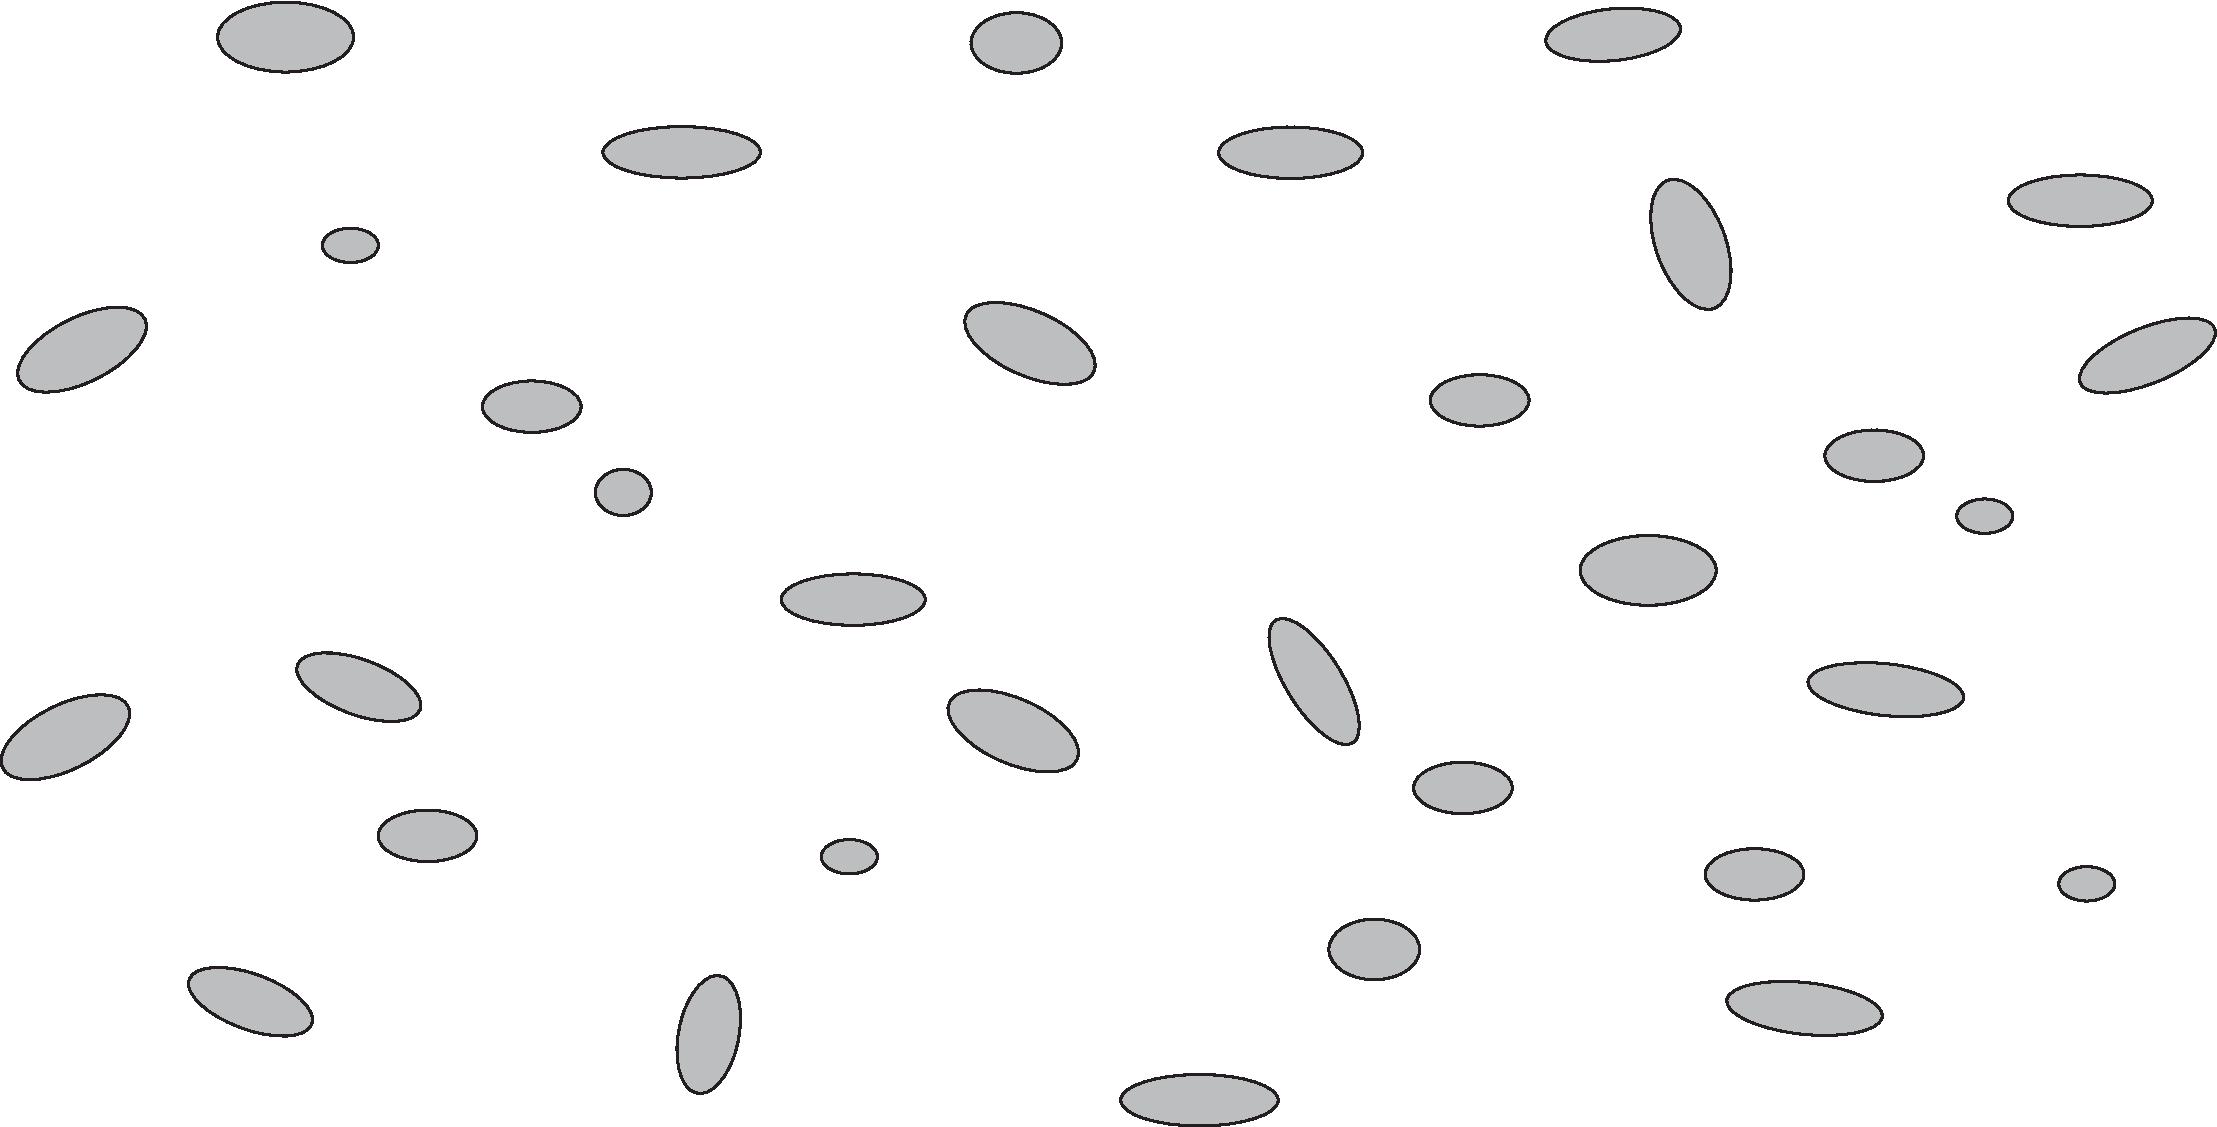
\includegraphics[scale=0.15,angle=0]{images/03-fig}
\end{center}
\begin{block}{}
Relatively rare events (streaming between clumps) will significantly affect the particle transport. The free-path distribution \textcolor{blue}{$p(s)$} will have a \textbf{nonexponential peak} for large \textcolor{blue}{$s$}.
\end{block}
}

%SLIDE4---------------------------------------------------------------------------------
\frame[c]{
	\frametitle{L\' evy flights}

	A L\' evy flight is a random walk in which the step-lengths have a probability distribution that is heavy-tailed:
\begin{center}
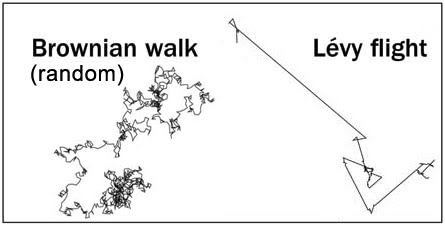
\includegraphics[scale=0.4,angle=0]{images/04-fig.jpg}
\end{center}
\begin{columns}
\column{6cm}
\begin{itemize}
\item L\' evy glasses
\item Astronomy
\item Cryptography
\end{itemize}
\column{6cm}
\begin{itemize}
\item Earthquake data analysis
\item Financial mathematics
\item Foraging hypothesis
\end{itemize}
\end{columns}
}

%SLIDE5---------------------------------------------------------------------------------
\frame[c]{
	\frametitle{Applications}
	\begin{figure}
	\centering
	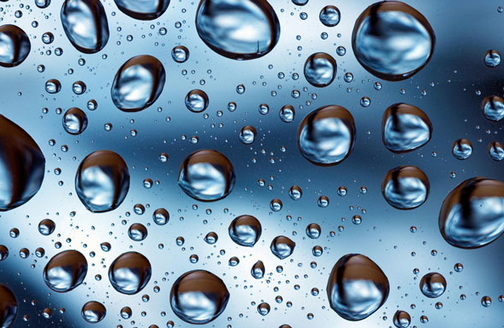
\includegraphics[scale=.3]{images/05-fig}
	\end{figure}	 
	%\pause
	\vspace{-4.7cm}
	\begin{figure}
	\centering
	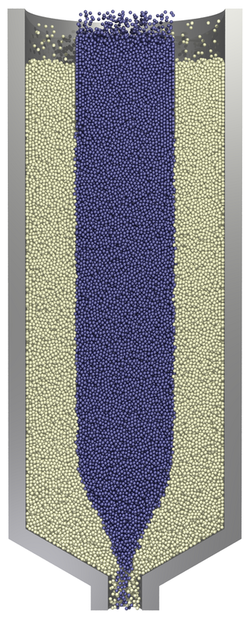
\includegraphics[scale=.2]{images/06-fig}\hfill
			\animategraphics[scale=.27,autoplay,loop]{7}{images/07-fig}{1}{12}
	\end{figure}	 
	}	 

%SLIDE06---------------------------------------------------------------------------------
\frame[c]{
	\frametitle{Path-length distribution}
	\small{
    In \textit{classical} particle transport, the incremental probability \textcolor{blue}{$dp$} that a particle will experience a collision while traveling an incremental path length \textcolor{blue}{$ds$} is:
   \[
   \textcolor{blue}{dp = \Sigma_t \, ds \;,}
   \]
where the total cross section \textcolor{blue}{$\Sigma_t$} is independent of
   \[
      \boxed{\textcolor{blue}{s}  = \text{the path length traveled since the previous interaction.}}
      \]
\pause
In the \textit{nonclassical} case we assume that \textcolor{blue}{$
    \Sigma_t = \Sigma_t(s) $},
and the conditional distribution function for distance-to-collision is
  \[ \boxed{\textcolor{blue}{
    p(s) = \Sigma_t(s) e^{ -\int_0^s \Sigma_t(s') ds' } \;. }}
  \]
 
  \begin{block}{}
{\bf Note}: in classical transport, \textcolor{blue}{$\Sigma_t(s) = \Sigma_t =$ constant}, and
  \[
   \textcolor{blue}{p(s) = \Sigma_t e^{ - \Sigma_t s } = \text{ exponential }} \;.  \nonumber
  \]
  \end{block}
}
}

%SLIDE07---------------------------------------------------------------------------------
\frame[c]{
	\frametitle{The Nonclassical linear Boltzmann equation}
	\footnotesize{
\begin{block}{Nonclassical transport}
   \begin{align} 
     \textcolor{blue}{ \frac{\partial \Psi }{\partial s} (\bm x, \bm \Omega, s)}
         + \textcolor{red}{\bm \Omega \cdot \bm \nabla \Psi}&\textcolor{red}{ (\bm x, \bm \Omega,s) + \Sigma_t(s) \Psi(\bm x, \bm \Omega,s) }
            \nonumber \\
         & \textcolor{teal}{=\frac{\delta(s)}{4\pi} \left[c\int_{4\pi}\int_0^{\infty} \Sigma_t(s')
            \Psi(\bm x, \bm \Omega', s') \, ds' d \Omega' + Q(\bm x)\right]}  \; \nonumber 
   \end{align}
\noindent
\end{block}
\begin{block}{Classical transport}
\[
\textcolor{red}{\bm\Omega\cdot\nabla\Psi(\bm x,\bm\Omega)}+
\textcolor{red}{\Sigma_t\Psi(\bm x, \bm\Omega)} = \textcolor{teal}{\frac{1}{4\pi}\left[c\Sigma_t\int_{4\pi}\Psi(\bm x,\bm\Omega')d\Omega'
+ Q(\bm x)\right]}
\]
\end{block}
%\pause
%\begin{columns}
%	\column{0.40\linewidth}
%	\begin{center}
%	\textcolor{blue}{$\begin{array}{r}\Sigma_t(s)=\\ \textcolor{white}{.}\end{array}$}\includegraphics[scale=.15]{question}
%	\end{center}
%	\column{0.09\linewidth}
%	%But, we know that	
%	\includegraphics[scale=.12]{arra}
%	\column{0.40\linewidth}
\textcolor{blue}{
\[
\Sigma_t(s) = \frac{p(s)}{1-\int_0^sp(s')ds'}\]}
%\end{columns}
}
}

%SLIDE08---------------------------------------------------------------------------------
\frame[c]{
	\frametitle{Thoughts...}
	
\begin{itemize}
\item Nonclassical transport requires one to know \textcolor{blue}{$\Sigma_t(s)$} (or \textcolor{blue}{$p(s)$}), which is not easy to obtain\vspace{10pt}
\item Nonclassical \textit{diffusion} is simpler: it only requires the first and second moments of \textcolor{blue}{$p(s)$} to be known\vspace{10pt}
\item Can we extend this result to obtain more accurate diffusion approximations? Maybe using something similar to the SP$_N$ approach?
\end{itemize}
}

%%%%%%%%%%%%%%%%%%%%%%%%%%%%%%%%%%%%%%%%%%%%%%%%%%%%%%
\section{\scshape Classical SP$_N$}
%SLIDE09---------------------------------------------------------------------------------
\frame[c]{
	\frametitle{P$_N$ Equations}
   Consider the planar (slab) geometry P$_N$ equations: for \textcolor{blue}{$l' = 0, 1, \dots$}, we have

\footnotesize{  
\textcolor{blue}{ 
\[
\left(\frac{l'+1}{2l'+1}\right)\frac{d}{d x}\phi_{l'+1}(x) + \left(\frac{l'}{2l'+1}\right)\frac{d}{d x}\phi_{l'-1}(x) + \Sigma_t(x) \phi_{l'} = \Sigma_{sl'}(x)\phi_{l'}(x) + s_{l'}(x)\:,
\]
}
}

\normalsize{
with 
\textcolor{blue}{
\[\phi_{-1}=0 \quad\text{ and }\quad\phi_{N+1} = 0 \quad\left(\text{ or }\quad\frac{d}{dx}\phi_{N+1}=0\,\right).
\]
}
The classical simplified P$_N$ equations (SP$_N$) can be obtained from the equation above in a heuristic way.
}
}

%SLIDE10---------------------------------------------------------------------------------
\frame[c]{
	\frametitle{``Heuristic'' Derivation of SP$_N$ Equations}
	\begin{center}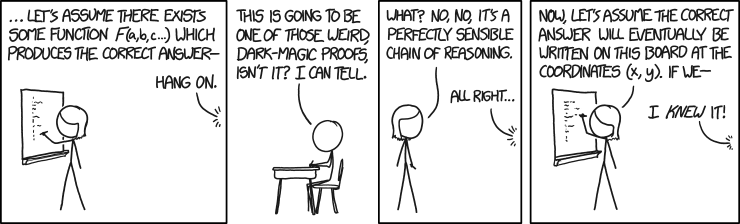
\includegraphics[scale=0.35]{images/08-fig}\end{center}
	\pause
\small{	
	First, for odd values of \textcolor{blue}{$l'$, $\phi_{l'}$} is replaced by a vector:
	\textcolor{blue}{
\[
\phi_{l'} \rightarrow \vec{\phi}_{l'} = (\phi_{l'}^x,\phi_{l'}^y,\phi_{l'}^z)^t\,.
\]
}

Then, in the even \textcolor{blue}{$l'$} equations the derivative in \textcolor{blue}{$x$} is replaced by a divergence: 
\textcolor{blue}{
\[
\frac{d}{dx} \rightarrow \nabla \cdot\,;
\]
}

and in the odd \textcolor{blue}{$l'$} equations the \textcolor{blue}{$x$} derivative is changed to a gradient: 
\textcolor{blue}{
\[
\frac{d}{dx} \rightarrow \nabla
\]
}
}
}

%SLIDE11---------------------------------------------------------------------------------
\frame[c]{
	\frametitle{``Heuristic'' Derivation of SP$_N$ Equations}
This allows us to write the first-order form of the SP$_N$ equations as 
\footnotesize{
\textcolor{blue}{
\begin{align*}
&\nabla \cdot \vec{\phi}_1 + \Sigma_a\phi_0 = s_0\,,\\
&\\
&\left(\frac{l'+1}{2l'+1}\right)\nabla\phi_{l'+1} + \left(\frac{l'}{2l'+1}\right)\nabla\phi_{l'-1} + \Sigma_t \vec{\phi}_{l'} = \Sigma_{sl'}\vec{\phi}_{
l'} + s_{l'}\:, \text{for odd $l'$,}\\
&\\
&\left(\frac{l'+1}{2l'+1}\right)\nabla\cdot\vec{\phi}_{l'+1} + \left(\frac{l'}{2l'+1}\right)\nabla\cdot\vec{\phi}_{l'-1} + \Sigma_t \phi_{l'} = \Sigma_{sl'}\phi_{l'} + s_{l'}\:, \text{for even $l'>0$.}
\end{align*}
}}
\pause
\normalsize{
We can get rid of the odd moments and rewrite them in their second-order form by using the relation
\textcolor{blue}{
\[
\vec{\phi}_{l'} = -\frac{1}{\Sigma_t-\Sigma_{sl'}}\left(\frac{l'}{2l'+1}\nabla\phi_{l'-1}+\frac{l'+1}{2l'+1}\nabla\phi_{l'+1}\right)\,.
\]
}
}
}

%SLIDE12---------------------------------------------------------------------------------
\frame[c]{
	\frametitle{Why SP$_N$?}
\small{
\begin{enumerate}
\item Mathematical structure is simpler: SP$_N$ are elliptic; P$_N$ are hyperbolic
\item The SP$_N$ equations can be understood as a ``super'' diffusion theory
\item The structure of the SP$_N$ equations is that of a coupled system of diffusion equations
\pause
\item Much simpler than P$_N$ in multidimensional problems (with fewer equations)
\item Simpler code implementation: just use/adapt a diffusion code!!
\pause
\item The SP$_N$ equations contain more ``transport physics'' than the diffusion equations.
\end{enumerate}
}
}


%SLIDE13---------------------------------------------------------------------------------
\frame[c]{
	\frametitle{Qualitative Behavior of SP$_N$ Equations}
\begin{center}
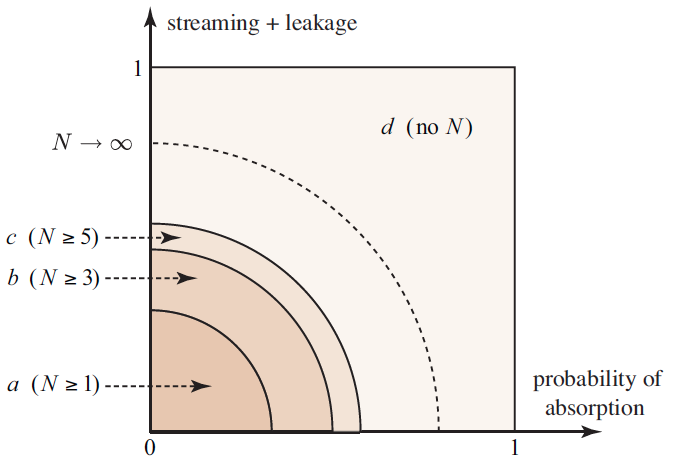
\includegraphics[scale=0.3]{images/09-fig}
\end{center}

The amounts of absorption and streaming/leakage are indicated on arbitrary scales ranging from 0 to 1.
}

%%%%%%%%%%%%%%%%%%%%%%%%%%%%%%%%%%%%%%%%%%%%%%%%%%%%%%
\section{\scshape Asymptotics}
%SLIDE14---------------------------------------------------------------------------------
\frame[c]{
	\frametitle{Asymptotic Analysis}
	\footnotesize{
Let us write the nonclassical Boltzmann equation in the mathematically equivalent form
\textcolor{blue}{
\bala
&\f{\partial \Psi}{\partial s}(s) + \uom \cdot \unab \Psi(s) + \Sigma_t(s)\Psi(s) = 0, \qquad s>0,\\
&\Psi(0) = \f{1}{4\pi}\left[\int_{4\pi}\int_0^\infty c\Sigma_t(s')\Psi(\ux,\uom',s')ds'd\Omega' + Q(\ux)\right].
\nala
}

Defining \textcolor{blue}{$0<\ep\ll 1$}, we perform the following scaling:
\textcolor{blue}{
\bala
\Sigma_t(s) &= \ep^{-1}\Sigma_t(s/\ep)\\
 c &= 1-\ep^2\kappa \\
 Q(\ux) &= \ep q(\ux)
 \nala
 }
where \textcolor{blue}{$\kappa$} and \textcolor{blue}{$q$} are \textcolor{blue}{$O(1)$}.

Under this scaling,
\textcolor{blue}{
\bala
\bl s^m\bg &=
%\ep^m\int_0^\infty \left(\f{s}{\ep}\right)^m \f{1}{\ep}\Sigma_t(s/\ep)e^{-\int_0^s\f{1}{\ep}\Sigma_t(s'/\ep)ds'}ds  \\ &=
\ep^m\int_0^\infty s^m\Sigma_t(s)e^{-\int_0^s\Sigma_t(s')ds'}ds = \ep^m\bl s^m\bg_\ep,
\nala
}
where \textcolor{blue}{$\bl s^m\bg_\ep$} is \textcolor{blue}{$O(1)$}.
}}

%SLIDE15---------------------------------------------------------------------------------
\frame[c]{
	\frametitle{Asymptotic Analysis}
\small{
Next, we define
\textcolor{blue}{
\bala
\psi(\ux,\uom,s)\equiv\f{\ep\sue}{e^{-\int_0^s\Sigma_t(s')ds'}}\Psi(\ux,\uom,\ep s).
\nala
}

This satisfies
\textcolor{blue}{
\bala
&\f{\partial \psi}{\partial s}(s) + \ep\uom \cdot \unab \psi(s)= 0, \qquad s>0,\\
&\psi(0) =  \f{1}{4\pi}\left[\int_{4\pi}\int_0^\infty (1-\ep^2\kappa)p(s')\psi(\ux,\uom',s')ds'd\Omega' + \ep^2 \sue q(\ux)\right],%\nonumber
\nala
}
and the classical scalar flux can be written as
\textcolor{blue}{
\bala
\Phi(\ux) = \int_{4\pi}\int_0^\infty \psi(\ux,\uom,s)\f{e^{-\int_0^s\Sigma_t(s')ds'}}{\sue}ds\: d\Omega.
\nala
}

We now integrate the first equation over \textcolor{blue}{$0<s'<s$}.
}}

%SLIDE16---------------------------------------------------------------------------------
\frame[c]{
	\frametitle{Asymptotic Analysis}

Using the ``initial condition'' in \textcolor{blue}{$s$}, we obtain
\textcolor{blue}{
\bala%\label{2.9}
&\left(I+\ep\uom\cdot\unab\int_0^s(\cdot)ds\right)\psi = \f{1}{4\pi}\left[\int_0^\infty (1-\ep^2\kappa)p(s')\vi(\ux,s')ds' + \ep^2\sue q\right],
\nala
}

where
\textcolor{blue}{
\bala
\vi(\ux,s) = \int_{4\pi}\psi(\ux,\uom,s)d\Omega.
\nala
}

Inverting the operator on the left-hand side of the above equation and expanding it in a power series, we obtain
\textcolor{blue}{
\bala
\psi &= \left(\sum_{n=0}^{\infty}(-\ep)^n\left(\uom\cdot\unab\int_0^s(\cdot)ds\right)^n\right) \times \\
&\qquad\qquad \left[\int_0^\infty \f{1-\ep^2\kappa}{4\pi}p(s')\vi(\ux,s')ds' + \ep^2\sue \f{q}{4\pi}\right].
\nala
}}

%SLIDE17---------------------------------------------------------------------------------
\frame[c]{
	\frametitle{Asymptotic Analysis}
Next we will need the identity 
\textcolor{blue}{
\bala
\f{1}{4\pi}\int_{4\pi}\left(\uom\cdot\unab\int_0^s(\cdot)ds\right)^nd\Omega = 
\f{1+(-1)^n}{2}\f{3^{n/2}}{n+1}\setb^{n/2},
\nala
}
for \textcolor{blue}{$n=0,1,2,...$} , where
\textcolor{blue}{
\bala
\setb &=\unab_0\left(\int_0^s(\cdot)ds\right)^2,\\
\unab_0&= \f{1}{3}\unab^2.
\nala
}

Integrating the nonclassical angluar flux over the unit sphere we obtain
\textcolor{blue}{
\bala
\vi &= \left(\sum_{n=0}^{\infty}\f{\ep^{2n}}{2n+1}(3\setb)^n\right)\left[\int_0^\infty (1-\ep^2\kappa)p(s')\vi(\ux,s')ds' + \ep^2\sue q\right].
\nala
}
}

%SLIDE18---------------------------------------------------------------------------------
\frame[c]{
	\frametitle{Asymptotic Analysis}
Inverting the operator on the right-hand side and once again expanding it in a power series, we get
\textcolor{blue}{
\bala
\left(I- \ep^2 \setb - \f{4\ep^4}{5}\setb^2 - \f{44\ep^6}{35}\setb^3 + O(\ep^8)\right)&\vi =\\
&\hspace{-5em}\int_0^\infty (1-\ep^2\kappa)p(s')\vi(\ux,s')ds' + \ep^2\sue q.
\nala
}
The solution of this equation is
\textcolor{blue}{
\bala
&\vi(\ux,s) = \left(I + \ep^2\f{s^2}{2!}\unab_0 + \f{9\ep^4}{5}\f{s^4}{4!}\unab_0^2 + \f{27\ep^6}{7}\f{s^6}{6!}\unab_0^3 + O(\ep^8)\right)\phi(\ux),%\nonumber
\nala
}
where 
\textcolor{blue}{
\bala
\phi(\ux) = {\sum_{n=0}^\infty  \ep^2\phi_{2n}(\ux)},
\nala
}
with \textcolor{blue}{$\phi_{2n}(\ux)$} undetermined at this point.
}

%SLIDE19---------------------------------------------------------------------------------
\frame[c]{
	\frametitle{Asymptotic Analysis}
\footnotesize{
We now multiply \textcolor{blue}{$\vi$} by \textcolor{blue}{$e^{-\int_0^s\Sigma_t(s')ds'}/\sue$}
and operate by \textcolor{blue}{$\int_0^\infty (\cdot) ds$}.
We obtain an expression for the scalar flux:
\textcolor{blue}{
\bala
\Phi(\ux) = &\left(I + \ep^2\f{\ste}{3!\sue}\unab_0 + \f{9\ep^4}{5}\f{\sce}{5!\sue}\unab_0^2 + \f{27\ep^6}{7}\f{\bl s^7\bg_\ep}{7!\sue}\unab_0^3 + O(\ep^8)\right)\phi(\ux). 
\nala
}

Moreover, we can write
\textcolor{blue}{
\bala
\int_0^\infty p(s)\vi(\ux,s)ds = \left(\sum_{n=0}^\infty\ep^{2n}U_n\unab_0^n \right)\Phi(\ux),
\nala
}
with \textcolor{blue}{$U_0 = 1$; $U_1= \f{\sde}{2!}-\f{\ste}{3!\sue};$
\bala
U_2 &= \f{9}{5}\left[\f{\sqe}{4!}-\f{\sce}{5!\sue}\right]-\f{\ste}{3!\sue}U_1;\\
U_3 &=\f{27}{7}\left[\f{\sse}{6!}-\f{\bl s^7\bg_\ep}{7!\sue}\right]-\f{9}{5}\f{\sce}{5!\sue}U_1-\f{\ste}{3!\sue}U_2;
\nala
}}
}

%SLIDE20---------------------------------------------------------------------------------
\frame[c]{
	\frametitle{Asymptotic Analysis}
We can now rewrite the whole equation as
\textcolor{blue}{
\bala
&\left(\sum_{n=0}^\infty \ep^{2n}V_n\unab_0^n\right)\Phi(\ux) = (1-\ep^2\kappa)\left(\sum_{n=0}^\infty\ep^{2n}U_n\unab_0^n \right)\Phi(\ux) + \ep^2\sue q(\ux),
\nala
}
where
\textcolor{blue}{
\bala
V_0 &= 1;\\
V_1&= -\f{\ste}{3!\sue}V_0;\\
V_2 &= -\f{9}{5}\f{\sce}{5!\sue}V_0 -\f{\ste}{3!\sue}V_1;\\
V_3 &= -\f{27}{7}\f{\bl s^7 \bg_\ep}{7!\sue}V_0 - \f{9}{5}\f{\sce}{5!\sue}V_1-\f{\ste}{3!\sue}V_2;\\
&... 
\nala
}
}

%SLIDE21---------------------------------------------------------------------------------
\frame[c]{
	\frametitle{Asymptotic Analysis}
	\small{
Finally, we rearrange the terms and get
\textcolor{blue}{
\bala
\boxed{\left(\sum_{n=0}^\infty \ep^{2n}\left[W_{n+1}\unab_0^{n+1}+\kappa U_n\unab_0^n\right]\right)\Phi(\ux) = \sue q(\ux),}
\nala
}
where \textcolor{blue}{$W_{n}=V_n-U_n$}.
\begin{center}
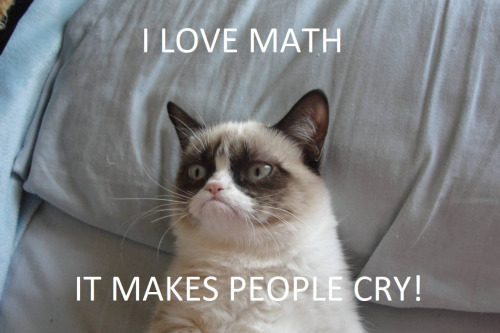
\includegraphics[scale=0.17]{images/10-fig.jpg}
\end{center}
\pause

\begin{itemize}
\item If we discard the terms of \textcolor{blue}{$O(\ep^{2n})$} in this equation, we obtain a partial differential equation for \textcolor{blue}{$\Phi(\ux)$} of order \textcolor{blue}{$2n$}
\item We will use this approach to explicitly derive the nonclassical SP$_1$, SP$_2$, and SP$_3$ equations
\item Higher-order equations can be derived by continuing to follow the same procedure
\end{itemize}
}
}

\section{\scshape Nonclassical SP$_N$}

%SLIDE22---------------------------------------------------------------------------------
\frame[c]{
	\frametitle{Nonclassical Diffusion (SP$_1$)}
Discarding the terms of \textcolor{blue}{$O(\ep^2)$} and reverting to the original unscaled parameters, we obtain
\bala
\textcolor{blue}{- \f{1}{6}\f{\sd}{\su}\unab^2\Phi(\ux) + \f{1-c}{\su}\Phi(\ux) = Q(\ux)},
\nala
which is the nonclassical diffusion equation. 

\pause
\vspace*{.5em}
If the free-path distribution \textcolor{blue}{$p(s)$} is an exponential, \textcolor{blue}{$\bl s^m\bg = m!\Sigma_t^{-m}$} and this equation reduces to the classical diffusion equation
\bala
\textcolor{blue}{- \f{1}{3\Sigma_t}\unab^2\Phi(\ux) + \Sigma_a\Phi(\ux) = Q(\ux)}.
\nala
}

%SLIDE23---------------------------------------------------------------------------------
\frame[c]{
	\frametitle{Nonclassical SP$_2$}
Discarding the terms of \textcolor{blue}{$O(\ep^4)$} and reverting to the original unscaled parameters, we obtain
\textcolor{blue}{
\bala
-\f{1}{6}\f{\sd}{\su}\unab^2 &\bigg[\Phi(\ux)+\lambda_1\left[(1-c)\Phi(\ux) - \su Q(\ux)\right]\bigg]+\\
 &\qquad\qquad\f{1-c}{\su} \big[1-\beta_1(1-c)\big]\Phi(\ux) =
\big[1-\beta_1(1-c)\big]Q(\ux),\nonumber
\nala
}
with \textcolor{blue}{$\lambda_1 = \f{3}{10}\f{\sq}{\sd^2} - \f{1}{3}\f{\st}{\su\sd}$} and 
\textcolor{blue}{$\beta_1 = \f{1}{3}\f{\st}{\su\sd} - 1$}.

\pause
If the free-path distribution \textcolor{blue}{$p(s)$} is an exponential, \textcolor{blue}{$\lambda_1 = \f{4}{5}$, $\beta_1=0$}, and this equation reduces to the classical SP$_2$ equation
\textcolor{blue}{
\bala
- \f{1}{3\Sigma_t}\unab^2&\left[\Phi(\ux) + \f{4}{5}\f{\Sigma_a\Phi(\ux)- Q(\ux)}{\Sigma_t}\right] + \Sigma_a\Phi(\ux) = Q(\ux).
\nala
}
}

%SLIDE24---------------------------------------------------------------------------------
\frame[c]{
	\frametitle{Nonclassical SP$_3$}
Discarding the terms of \textcolor{blue}{$O(\ep^6)$} and reverting to the original unscaled parameters, we obtain
\textcolor{blue}{
\bala
&-\f{1}{6}\f{\sd}{\su}\unab^2\bigg[\big[1+\beta_1(1-c)\big]\Phi(\ux) + 2\nu(\ux)\bigg] + \f{1-c}{\su}\Phi(\ux) = Q(\ux),\\
&-\f{1}{6}\f{\sd}{\su}\unab^2\left[\f{\lambda_1}{2}\Phi(\ux)+\lambda_2\nu(\ux)\right]+\f{1-\beta_2(1-c)}{\su}\nu(\ux) = 0,
\nala
}
with
\textcolor{blue}{
\bala
\lambda_2 =& \f{1}{10\sd\st-9\su\sq } \left[\f{9}{5}\sc - \f{27}{21}\f{\su\ss}{\sd} + 3\f{\st\sq}{\sd} - \f{10}{3} \f{\st^2}{\su}\right],\\
\beta_2 =& \f{1}{10\sde\ste-9\sue\sqe}\left[\f{10}{3}\f{\ste^2}{\sue} - \f{9}{5}\sce\right]-1.
\nala
}
}

%SLIDE25---------------------------------------------------------------------------------
\frame[c]{
	\frametitle{Nonclassical SP$_3$}
If the free-path distribution \textcolor{blue}{$p(s)$} is an exponential, \textcolor{blue}{$\lambda_2 = \f{11}{7}$, $\beta_2=0$}, and these equations reduce to the classical SP$_3$ equations
\textcolor{blue}{
\bala
-\f{1}{3\Sigma_t}\unab^2\bigg[\Phi(\ux) + 2\nu(\ux)\bigg] + \Sigma_a\Phi(\ux) = Q(\ux),\\
-\f{1}{3\Sigma_t}\unab^2\left[\f{2}{5}\Phi(\ux)+\f{11}{7}\nu(\ux)\right]+\Sigma_t\nu(\ux) = 0.
\nala
}
}


%SLIDE26---------------------------------------------------------------------------------
\frame[c]{
	\frametitle{Regarding Boundary Conditions...}
%\pause	
\begin{center}

\includegraphics[scale=0.3]{images/11-fig.jpg}	
\end{center}	
\pause

\begin{itemize}
\item Nonclassical transport boundary conditions are not yet well-defined for the ``backward'' nonclassical equation
\item The asymptotic analysis for the classical SP$_N$ equations does not yield boundary conditions...
%\pause
and neither does the present one  
\end{itemize}
\pause	

\textcolor{red}{Solution:} manipulate the nonclassical SP$_N$ equations into a classical form and use classical (Marshak) boundary conditions.
}


%SLIDE27---------------------------------------------------------------------------------
\frame[c]{
	\frametitle{Nonclassical Diffusion with Vacuum Boundaries}
	The nonclassical diffusion equation is 
\textcolor{blue}{
	\bala
\textcolor{blue}{- \f{1}{6}\f{\sd}{\su}\unab^2\Phi(\ux) + \f{1-c}{\su}\Phi(\ux) = Q(\ux)}.
\nala
}
We define
\textcolor{blue}{
\bala
\wst &= 2\f{\su}{\sd}, \qquad \wsa = \f{1-c}{\su},
\nala
}

\pause
and rewrite it as a classical diffusion equation, for which we use Marshak boundary conditions:
\textcolor{blue}{
\bala
- \f{1}{3\wst}\unab^2\Phi(\ux) + \wsa\Phi(\ux) &= Q(\ux),\\
\text{\textcolor{black}{B.C.:}}\qquad \f{1}{2}\Phi(\ux) -\f{1}{3\wst}\vec\un\cdot\unab\Phi(\ux) &= 0.
\nala
}
}


%SLIDE28---------------------------------------------------------------------------------
\frame[c]{
	\frametitle{Nonclassical SP$_2$ with Vacuum Boundaries}
	\textcolor{blue}{
\bala
- \f{1}{3\wst}\unab^2\widehat\Phi(\ux) + \wsa\widehat\Phi(\ux) &= \wq(\ux),\\
\text{\textcolor{black}{B.C.:}}\qquad \f{1}{2}\widehat\Phi(\ux) -\f{1}{3\wst}\vec\un\cdot\unab\widehat\Phi(\ux) &= 0,
\nala
}
with
\textcolor{blue}{
\bala
\wst &= 2\f{\su}{\sd},&\wsa &=\f{(1-c)}{\su} \f{1-\beta_1(1-c)}{1+\lambda_1(1-c)},\\
\wq(\ux) &= \f{1-\beta_1(1-c)}{1+\lambda_1(1-c)} Q(\ux),&\Phi(\ux) &= \frac{\widehat\Phi(\ux) + \lambda_1\su Q(\ux)}{1+\lambda_1(1-c)}.
\nala
}
}


%SLIDE29---------------------------------------------------------------------------------
\frame[c]{
	\frametitle{Nonclassical SP$_3$ with Vacuum Boundaries}
	\footnotesize{
	\textcolor{blue}{
\bala
&-\f{1}{3\wst}\unab^2\big[\Phi(\ux) + 2\widehat\Phi_2(\ux)\big] + \wsa\Phi(\ux) = \wq(\ux),\\
&-\f{1}{3\wst}\unab^2\left[\f{2}{5}\Phi(\ux)+\left(\f{4}{5}+\f{27\wst}{35\widehat\Sigma_3}\right)\widehat\Phi_2(\ux)\right]+\widehat\Sigma_2\widehat\Phi_2(\ux) = 0,\\
&\text{\textcolor{black}{B.C.:}}\qquad\f{1}{2}\Phi(\ux)-\f{1}{3\wst}\vec\un\cdot\unab\Phi(\ux) -\f{2}{3\wst}\vec\un\cdot\unab\widehat\Phi_2(\ux) +\f{5}{8}\widehat\Phi_2(\ux) = 0,\\
&\text{\textcolor{black}{B.C.:}}\qquad-\f{1}{8}\Phi(\ux) +\f{5}{8}\widehat\Phi_2(\ux) -\f{3}{7\widehat\Sigma_3} \vec\un\cdot\unab\widehat\Phi_2(\ux) = 0,
\nala
}
with
\textcolor{blue}{
\bala
\widehat\Phi_2(\ux) &= \f{\nu(\ux)}{1+\beta_1(1-c)}, &\wst &= 2\f{\su}{\sd},\\
\wsa &=\f{(1-c)}{\su} \f{1}{1+\beta_1(1-c)}, &\wq(\ux) &= \f{Q(\ux)}{1+\beta_1(1-c)},\\
\widehat\Sigma_2 &= \f{4\left[1+\beta_1(1-c)\right]\left[1-\beta_2(1-c)\right]}{5\lambda_1\su}, &\widehat\Sigma_3 &= \f{27}{28}\f{\lambda_1\wst}{\lambda_2\left[1+\beta_1(1-c)\right]-\lambda_1}.
\nala
}
}}

%%%%%%%%%%%%%%%%%%%%%%%%%%%%%%%%%%%%%%%%%%%%%%%%%%%%%%
\section{\scshape Numerics}

%SLIDE30---------------------------------------------------------------------------------
\frame[c]{
	\frametitle{1-D random periodic media}
We consider a 1-D physical system consisting of alternating layers of solid and void, periodically arranged:
\begin{center}
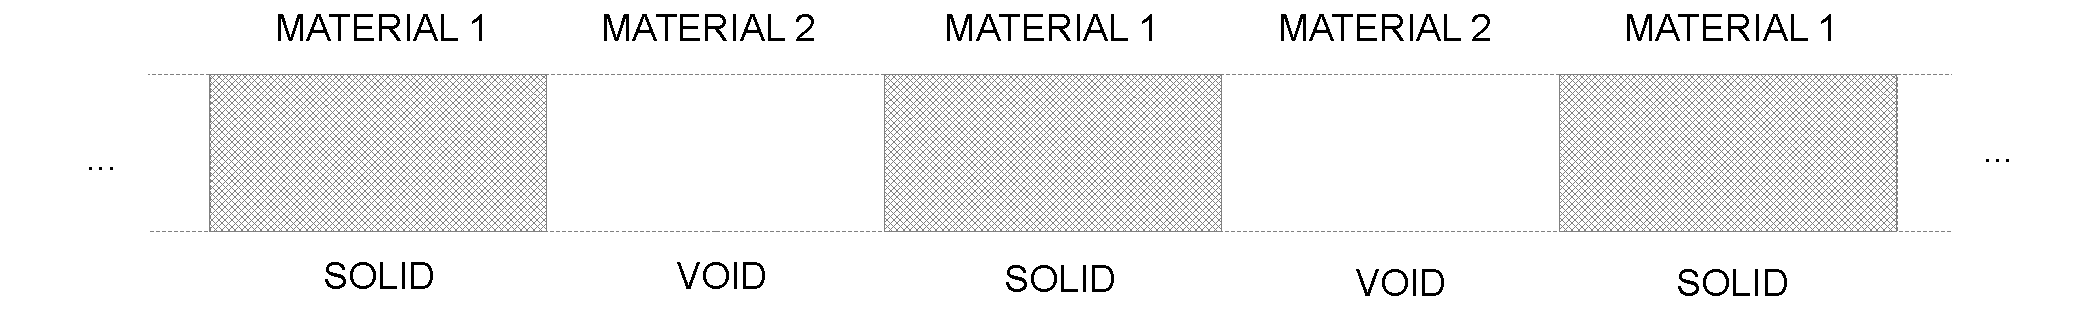
\includegraphics[scale=0.3,angle=0]{images/12-fig.pdf}
\end{center}
\begin{itemize}
\item layers of material 1 and 2 have thicknesses \textcolor{blue}{$\ell_1$} and \textcolor{blue}{$\ell_2$}, respectively; (period \textcolor{blue}{$\ell=\ell_1+\ell_2$})
\item the origin (\textcolor{blue}{$x=0$}) is {\em randomly placed} in the periodic system \footnotesize{(this is equivalent to randomly placing the system in the infinite line $-\infty < x < \infty$)}
\normalsize
\item the probability \textcolor{blue}{$P_i$} of finding material \textcolor{blue}{$i$} in a given point \textcolor{blue}{$x$} is \textcolor{blue}{$\ell_i/(\ell_1+\ell_2)$}
\end{itemize}
}


%SLIDE31---------------------------------------------------------------------------------
\frame[c]{
	\frametitle{The Path-length distribution function}
\scriptsize{
$\bigstar$ $\boldsymbol{\ell_1<\ell_2}:$
\[
\textcolor{blue}{
p(\mu,s)=  \left\{
\begin{array}{ll}
\frac{\Sigma_{t1}}{\ell_1}(n\ell+\ell_1-s|\mu|)e^{-\Sigma_{t1}(s-n\ell_2/|\mu|)}, & \text{if } n\ell\leq s|\mu|\leq n\ell+\ell_1
\\
0, & \text{if } n\ell+\ell_1\leq s|\mu|\leq n\ell+\ell_2 \\
\frac{\Sigma_{t1}}{\ell_1}(s|\mu|-n\ell+\ell_2)e^{-\Sigma_{t1}[s-(n+1)\ell_2/|\mu|)]}, & \text{if } n\ell+\ell_2\leq s|\mu|\leq (n+1)\ell
\end{array} 
\right. \nonumber
}
\pause
\]
$\bigstar$ $\boldsymbol{\ell_1=\ell_2}:$
\[
\textcolor{blue}{
p(\mu,s)=  \left\{
\begin{array}{ll}
\frac{\Sigma_{t1}}{\ell_1}(n\ell+\ell_1-s|\mu|)e^{-\Sigma_{t1}(s-n\ell_2/|\mu|)}, & \text{if } n\ell\leq s|\mu|\leq n\ell+\ell_1
\\
\frac{\Sigma_{t1}}{\ell_1}(s|\mu|-n\ell+\ell_2)e^{-\Sigma_{t1}[s-(n+1)\ell_2/|\mu|)]}, & \text{if } n\ell+\ell_2\leq s|\mu|\leq (n+1)\ell
\end{array} 
\right. \nonumber
}
\]
\pause
$\bigstar$ $\boldsymbol{\ell_1>\ell_2}:$
\[
\textcolor{blue}{
p(\mu,s)=  \left\{
\begin{array}{ll}
\frac{\Sigma_{t1}}{\ell_1}(n\ell+\ell_1-s|\mu|)e^{-\Sigma_{t1}(s-n\ell_2/|\mu|)}, & \text{if } n\ell\leq s|\mu|\leq n\ell+\ell_2
\\
\frac{\Sigma_{t1}}{\ell_1}[(n\ell+\ell_2-s|\mu|)(1-e^{\Sigma_{t1}\ell_2/|\mu|}) \hspace{1.3cm}, & \text{if } n\ell+\ell_2\leq s|\mu|\leq n\ell+\ell_1\\
\hspace{2,5cm}+\ell_1-\ell_2]e^{-\Sigma_{t1}(s-n\ell_2/|\mu|)} & \\
\frac{\Sigma_{t1}}{\ell_1}(s|\mu|-n\ell+\ell_2)e^{-\Sigma_{t1}[s-(n+1)\ell_2/|\mu|)]}, & \text{if } n\ell+\ell_1\leq s|\mu|\leq (n+1)\ell
\end{array} 
\right. \nonumber
}
\]


}
}

%SLIDE32---------------------------------------------------------------------------------
\frame[c]{
	\frametitle{$p(\mu=1,s)$ for $\Sigma_{t1}=1$, with $\ell_1=\ell_2=1$ }
	\scriptsize{	
\textcolor{blue}{
}
}
	\begin{center}
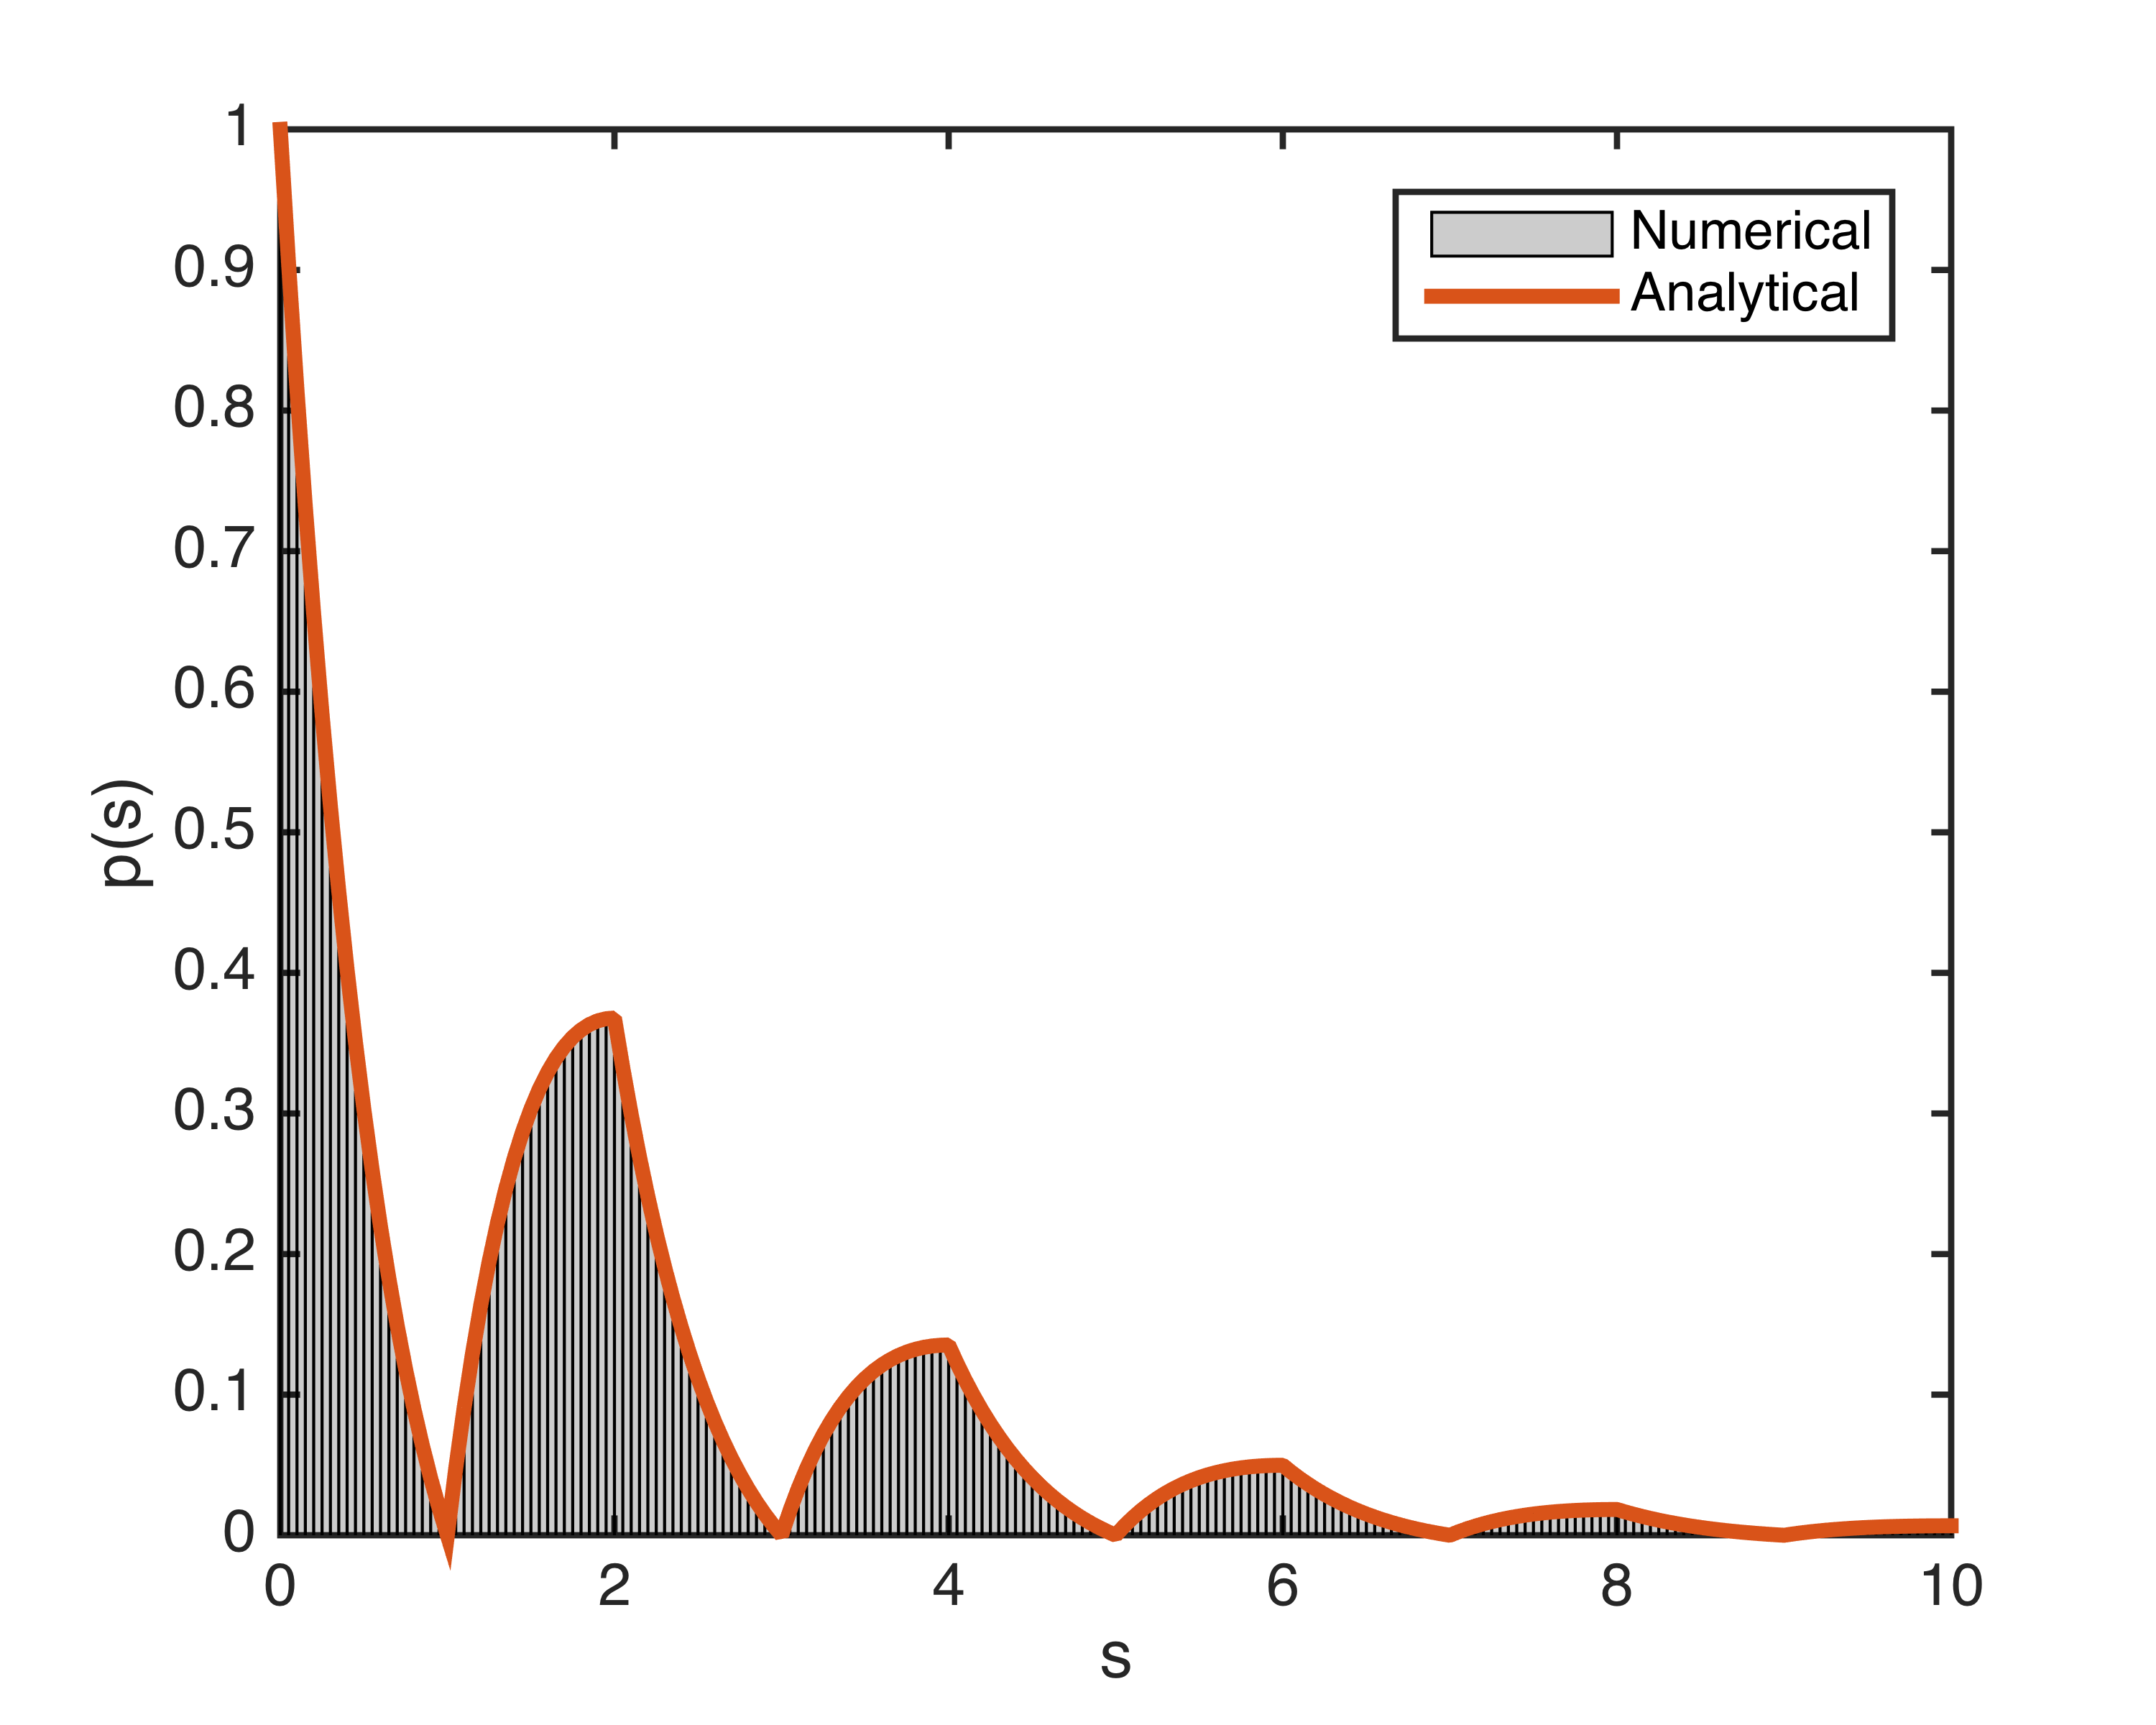
\includegraphics[scale=0.7,angle=0]{images/13-fig}
\end{center}
}

\frame[c]{
\setcounter{framenumber}{32}
	\frametitle{$p(\mu=1,s)$ for $\Sigma_{t1}=1$, with $\ell_1=\ell_2=1$}
%	\hspace{-17pt}
%\includegraphics[scale=0.17,angle=0]{pathlengthdistribution.pdf}\hspace{-29pt}
	\begin{center}
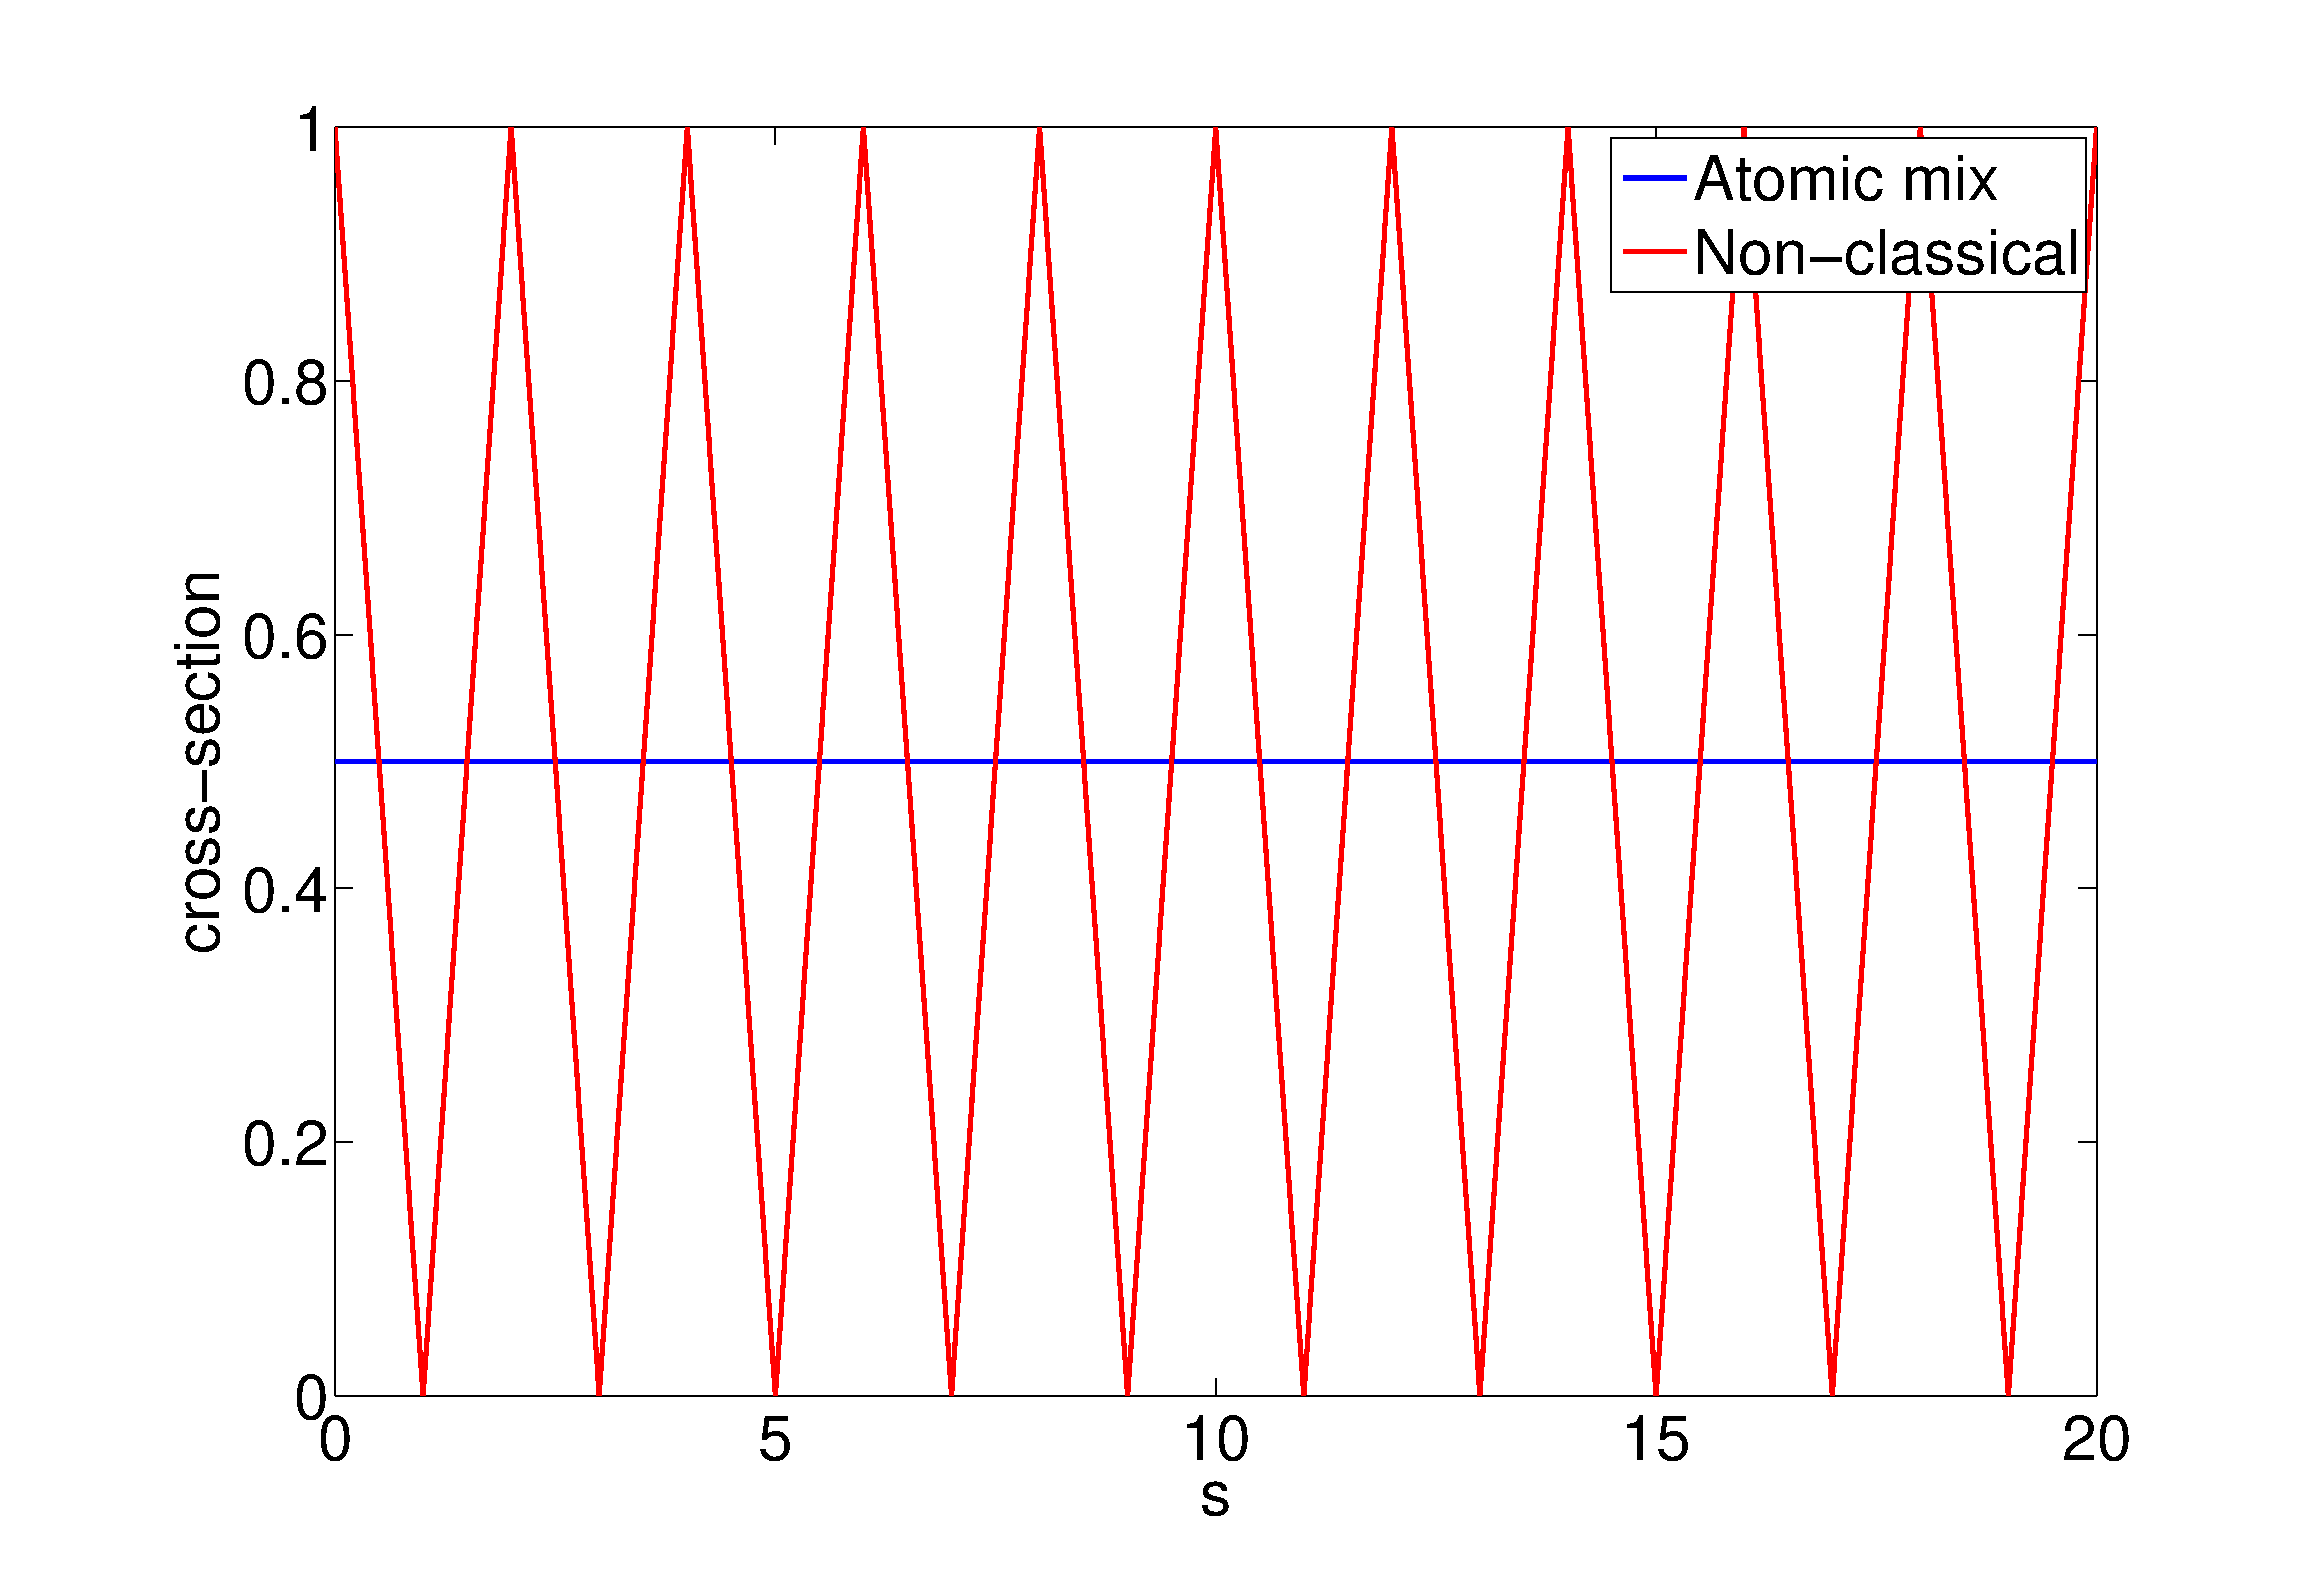
\includegraphics[scale=0.23,angle=0]{images/14-fig.pdf}
\end{center}
}


%SLIDE33---------------------------------------------------------------------------------
\frame[c]{
	\frametitle{1-D diffusive system}
\begin{center}
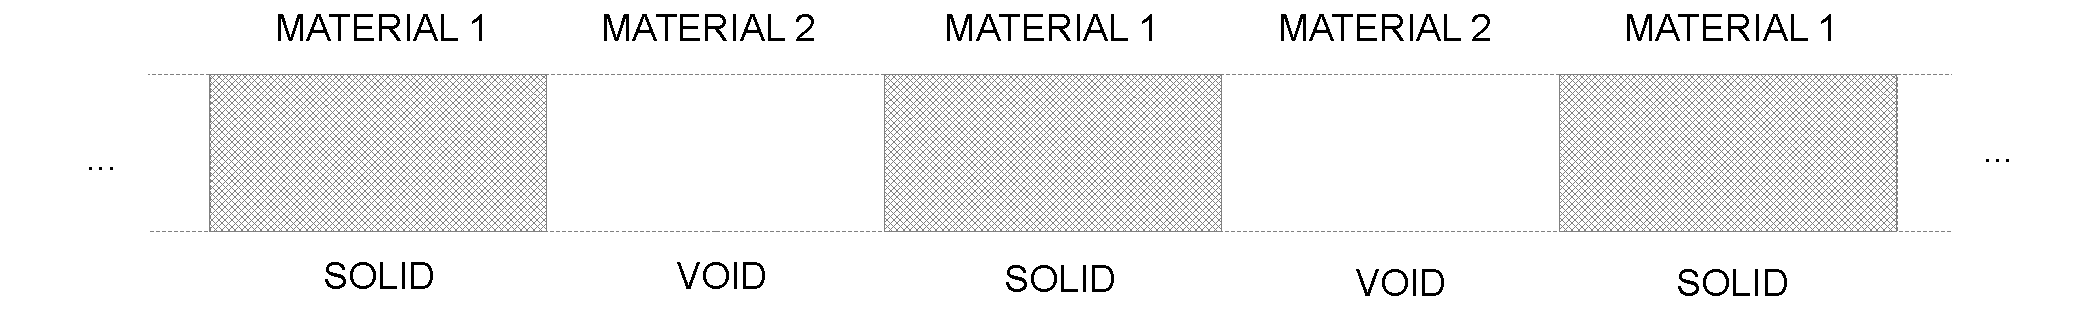
\includegraphics[scale=0.3,angle=0]{images/12-fig.pdf}
\end{center}
\begin{itemize}
\item Slab geometry
\item Isotropic scattering
\item Vacuum boundaries
\item Isotropic source
\item We define \textcolor{blue}{$M=\varepsilon^{-1}$}, and
   \begin{itemize}
   \item \textcolor{blue}{$\ell_1 = \ell_2 = 0.5$} $\Longrightarrow$ \textcolor{blue}{$\ell=1$}\vspace{3pt}
   \item \textcolor{blue}{$-M\leq x\leq M$} $\Longrightarrow$ \textcolor{blue}{$\ell M = O(\varepsilon^{-1}) $}\vspace{3pt}
   \item \textcolor{blue}{$\Sigma_{t1} = 1 = O(1)$} \vspace{3pt}
   \item \textcolor{blue}{$1-c = 0.1\times M^{-2} = O(\varepsilon^2) $} \vspace{3pt}
   \item \textcolor{blue}{$Q_1= 0.2\times M^{-2} = O(\varepsilon^2)$} 
    \end{itemize}
    \end{itemize}


}

%SLIDE34---------------------------------------------------------------------------------
\frame[c]{
	\frametitle{Error Estimates at $x=0$}
	\begin{center}
\includegraphics[scale=0.7,angle=0]{images/15-fig.eps}
\end{center}
}


%%%%%%%%%%%%%%%%%%%%%%%%%%%%%%%%%%%%%%%%%%%%%%%%%%%%%%
\section{\scshape Discussion}

%SLIDE35---------------------------------------------------------------------------------

\begin{frame}[fragile]{Discussion}
\begin{enumerate}
\item The nonclassical SP$_N$ equations provide more accurate diffusion approximations to nonclassical transport.
\item  However, they require all the moments of the \textcolor{blue}{$p(s)$} up to $2N$ to exist.
\item They can be manipulated into a set of \textit{classical} SP$_N$ equations with modified parameters.
\item Therefore, they can be implemented in already existing SP$_N$ codes.
\end{enumerate}
\pause

\textbf{Immediate things to do:}
\begin{itemize}
\item Perform a complete analysis of these results in nonclassical multi-dimensional systems.
\item Extend the analysis to angular dependent free-path distributions \textcolor{blue}{$p(\uom,s)$}.
%(the case of slab geometry)
\item Extend the analysis to anisotropic scattering.
\end{itemize}
\end{frame}


%SLIDE36---------------------------------------------------------------------------------	
	\frame[c]{\frametitle{Thank you for your attention!!!}  
%	\begin{columns}
%	\column{0.40\linewidth}
%	\begin{center}
%		\Large{Where to find me:}
%		\end{center}
%		\vspace{0.3cm}
%		\normalsize
%		\begin{itemize}
%		\item Website: \textcolor{blue}{\textbf{ricvasques.github.io}}
%		\item Email: \textcolor{blue}{\textbf{rvasques@berkeley.edu}}
%		\item GitHub: \textcolor{blue}{\textbf{github.com/ricvasques}}
%		\item Twitter:\\ \textcolor{blue}{\textbf{@Nuclear\_mat}}
%		\end{itemize}
%	\column{0.55\linewidth}
\begin{center}
\huge{Questions?}
\end{center}
\begin{figure}
	\centering
	
\includegraphics[scale=0.7]{images/16-fig.jpg}
		\end{figure}			
%		\end{columns}
	}	
	


\end{document}

